\documentclass{article}
\usepackage{graphicx}
\usepackage{amsmath}
\usepackage{hyperref}
\usepackage{algorithmic}

\title{CS121 Parallel Computing CUDA Lab: Cuckoo Hashing}
\author{Leshi Li 2023533001}
\date{January 10, 2025}

\begin{document}

\maketitle

\section{Introduction}

In this lab, I implement the parallel version of Cuckoo Hashing algorithm using CUDA and implement the sequential version of it for comparison.

\section{Algorithm}

The parallel Cuckoo Hashing algorithm implemented using CUDA consists of the following components:

\subsection{Hash Functions}
Since Cuckoo Hashing requires rehashing, I choose three different hash methods which can be seeded with random values to produce different hash function sets.
\begin{itemize}
    \item \textbf{Jenkins one-at-a-time hash}: This hash function processes the key byte by byte and combines it with a seed to produce a hash value.
    \item \textbf{FNV-1a hash}: This hash function uses the FNV-1a algorithm, which is a variant of the Fowler-Noll-Vo hash function, combined with a seed.
    \item \textbf{MurmurHash3}: This hash function uses the MurmurHash3 algorithm, which is known for its good distribution and performance, combined with a seed.
\end{itemize}

\subsection{Insertion}
The insertion process involves placing keys into the hash table using the available hash functions. If a collision occurs (i.e., the position is already occupied), the existing key is evicted and reinserted using the next hash function. This process continues until the key is placed in an empty slot or the maximum number of iterations is reached. If the maximum number of iterations is reached, a rehash is triggered with a new seed.

\subsection{Lookup}
The lookup process involves checking the positions determined by the hash functions to see if the key is present in any of them. If the key is found, the result is marked as true; otherwise, it is marked as false.

\subsection{Rehashing}
Rehashing is performed when the insertion process fails to place a key after the maximum number of iterations. A new seed is generated, and all keys are reinserted into the hash table. This process is repeated until all keys are successfully inserted or the maximum rehash depth is reached, in which case the insertion process is considered to have failed.

\subsection{CUDA Kernels}
Two CUDA kernels are used in the implementation:
\begin{itemize}
    \item \textbf{cuckooHashInsert}: This kernel performs the insertion of keys into the hash table in parallel. Each thread handles the insertion of one key. It uses \verb|atomicExch()| to handle the eviction of existing keys.
    \item \textbf{cuckooHashLookup}: This kernel performs the lookup of keys in the hash table in parallel. Each thread handles the lookup of one key.
\end{itemize}

\section{Benchmark Configs}

I run the four experiments in the lab handout.
I run the benchmark on 
\begin{itemize}
    \item OS: Ubuntu 22.04.4 LTS
    \item CPU: 13th Gen Intel(R) Core(TM) i9-13900HX
    \item GPU: NVIDIA GeForce RTX 4060
\end{itemize}

\section{Experiments}

\begin{itemize}
    \item \textbf{Experiment 1}: Create a hash table of $size=2^{25}$ in GPU global memory, where each table entry stores a
    32-bit integer. Insert a set of $n=2^{24}$ random integer keys into the hash table, for s =
    10,11, … 24.
    \item \textbf{Experiment 2}: Insert a set of $n=2^{24}$ random keys into a hash table of size $size=2^{25}$, then perform lookups
    for the following sets of keys $S_i$, where
    (100 - 10i) percent of the keys are randomly chosen from S, and the remainder are
    random 32-bit keys.
    \item \textbf{Experiment 3}: Fix a set of $n=2^{24}$ random keys, and measure the time to insert the keys into hash
    tables of sizes 1.1, 1.2, … , 2. Also, measure the insertion times for hash tables of
    sizes 1.01, 1.02 and 1.05. Terminate the experiment if it takes too long and report
    the time used.
    \item \textbf{Experiment 4}: Using $n=2^{24}$ random keys and a hash table of size 1.4, experiment with different
    bounds on the maximum length of an eviction chain before restarting. Which bound
    gives the best running time for constructing the hash table? Note however you are not
    required to find the optimal bound.
\end{itemize}

\subsection{Experiment 1}

The MOPs of $t=2$ and $t=3$ hash functions are very similar, since the number of keys is relatively less than the size of the hash table, and evictions happen relatively less frequently.

\subsection{Experiment 2}

The MOP of $t=2$ hash functions is higher than that of $t=3$ hash functions, since less hash functions are used for lookups. The MOP decreases as the percentage of random generated keys increases, since the lookup process is more likely to fail.

\subsection{Experiment 3}

When $t=2$, both the CUDA and sequential implementations suffer from the rehashing failure when the hash table is too small (size $< 1.1n$). When $t=3$, the CUDA implementation is more robust and can handle smaller hash tables. The CUDA implementation is faster than the sequential implementation for all hash table sizes.

\subsection{Experiment 4}

In this case, the MOP has relatively larger distribution, and are less sensitive to eviction chain bounds. That's because the hash table size if relatively larger, and less rehashing is needed.

\begin{figure}[h!]
    \centering
    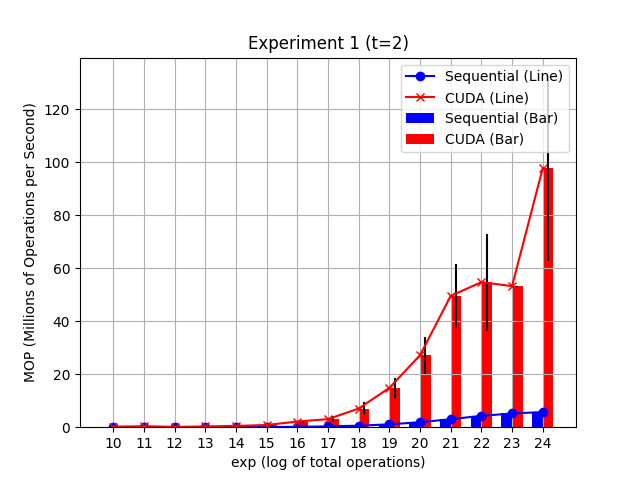
\includegraphics[width=\textwidth]{../figs/experiment1_t2.png}
    \caption{Experiment 1 with 2 hash functions}
\end{figure}

\begin{figure}[h!]
    \centering
    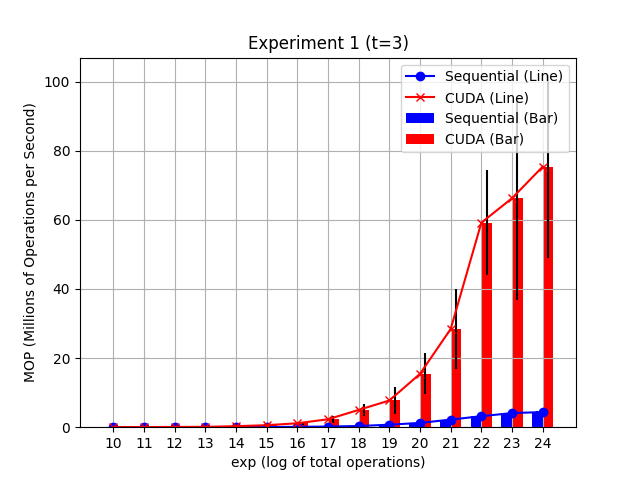
\includegraphics[width=\textwidth]{../figs/experiment1_t3.png}
    \caption{Experiment 1 with 3 hash functions}
\end{figure}

\begin{figure}[h!]
    \centering
    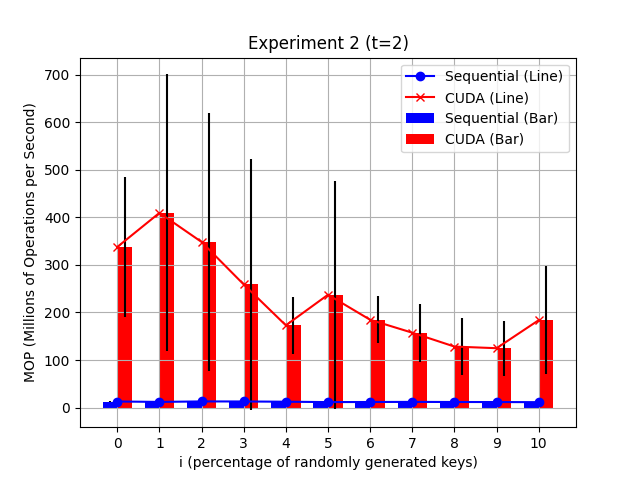
\includegraphics[width=\textwidth]{../figs/experiment2_t2.png}
    \caption{Experiment 2 with 2 hash functions}
\end{figure}

\begin{figure}[h!]
    \centering
    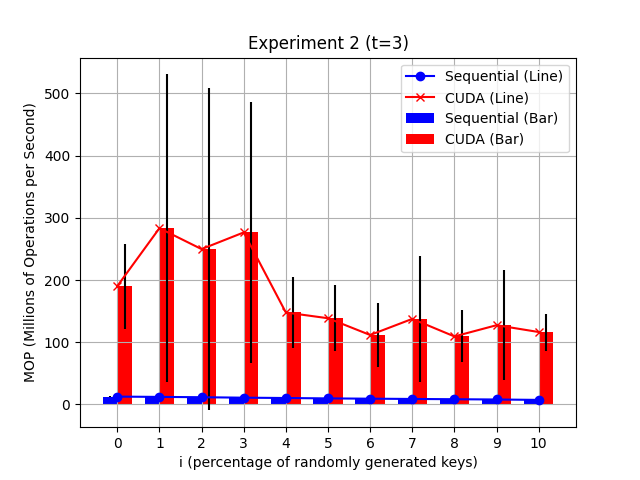
\includegraphics[width=\textwidth]{../figs/experiment2_t3.png}
    \caption{Experiment 2 with 3 hash functions}
\end{figure}

\begin{figure}[h!]
    \centering
    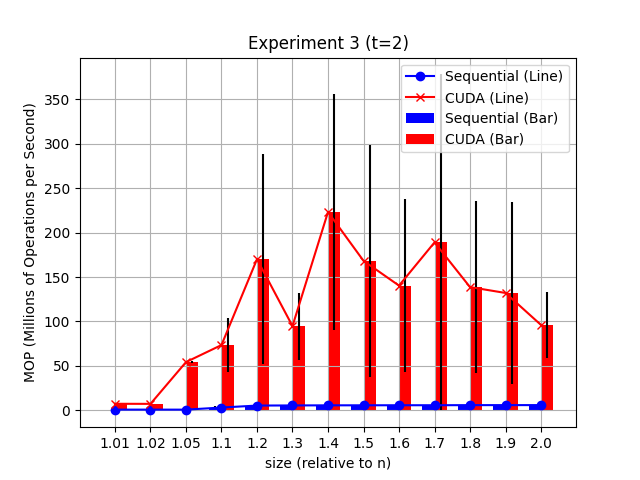
\includegraphics[width=\textwidth]{../figs/experiment3_t2.png}
    \caption{Experiment 3 with 2 hash functions}
\end{figure}

\begin{figure}[h!]
    \centering
    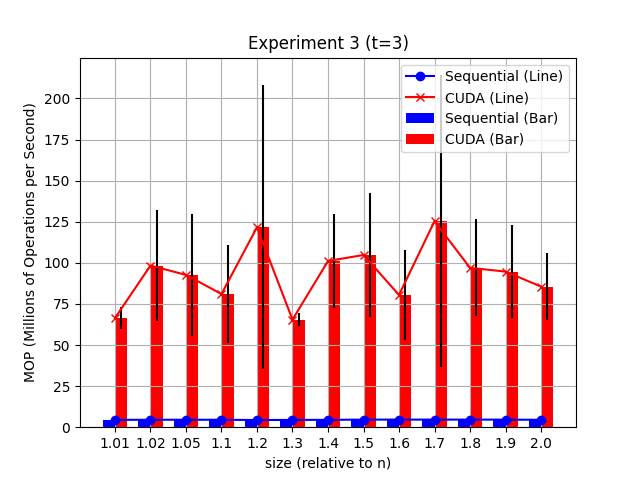
\includegraphics[width=\textwidth]{../figs/experiment3_t3.png}
    \caption{Experiment 3 with 3 hash functions}
\end{figure}

\begin{figure}[h!]
    \centering
    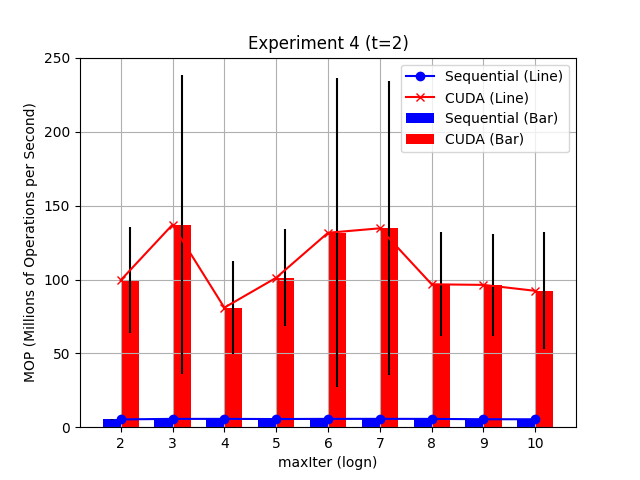
\includegraphics[width=\textwidth]{../figs/experiment4_t2.png}
    \caption{Experiment 4 with 2 hash functions}
\end{figure}

\begin{figure}[h!]
    \centering
    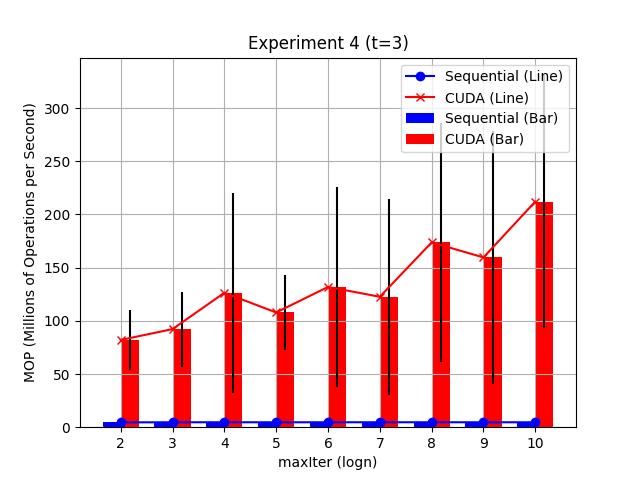
\includegraphics[width=\textwidth]{../figs/experiment4_t3.png}
    \caption{Experiment 4 with 3 hash functions}
\end{figure}

\end{document}
